\section{Main Content}
\subsection*{Top Level Architecture of Network Device}
\begin{frame}
    \frametitle{Basic Overview}
    \framesubtitle{Published in [MICPRO16] journal}
    %
    \begin{itemize}
        \fitem Current HLS tools are sensitive to provided input
        \fitem Controlled mapping process
        \begin{itemize}
            \fitem We can control the architecture generation process
            \fitem Easier to sustain parameters of generated network device (frequency, consumed resources)
        \end{itemize}
       
        \fitem The most modern abstract language is used (P4; since 2013)
        \fitem The mapping requires:
        \begin{enumerate}
            \fitem Modular target architecture of high-speed network device
            \fitem Identification of building macro blocks which are combination of optimized hand-written and generated code
        \end{enumerate}
        
        \fitem This approach allows:
        \begin{enumerate}
            \fitem Minimization of suboptimal input from the user
            \fitem Keep the quality of generated code (compared to hand-written)
            \fitem Rapid prototyping of high-speed network devices
            \begin{itemize}
                \fitem Many lines of HDL code are generated in short time
            \end{itemize}
        \end{enumerate}
    \end{itemize}
\end{frame}

\begin{frame}
    \frametitle{Use Case Study}
    \framesubtitle{Generated Code vs. Total Lines of Code}
    
    \begin{enumerate}
        \fitem \textbf{IPv4 Filter} --- filtering of packets is based on the IPv4 address, the non-IP traffic is dropped
        \fitem \textbf{IPv4+IPv6 Filter}  --- extends the IPv4 Filter with further support of IPv6 protocol, the non-IP traffic is dropped
        \fitem \textbf{Full Filter} --- extends the IPv4+IPv6 Filter with further support of tagging (VLAN and MPLS)
    \end{enumerate}
    
    
    \begin{table}
        \footnotesize
        \centering
        \begin{tabular}{|l||c|c||c|c|}
            \hline
            \T \textbf{Project} & \textbf{P4 lines} & \textbf{Time\,[s]} & \textbf{Generated lines} & \textbf{Total lines} \\ \hline\hline
            \T IPv4 Filter      &        91         &       1.574        &           6283           &        24791         \\
            IPv4+IPv6 Filter    &        129        &       1.818        &           9888           &        28396         \\
            Full Filter         &        212        &       1.929        &          13824           &        32332         \\ \hline
        \end{tabular}
    \end{table}
    
    \begin{itemize}
        \footnotesize
        \fitem \textbf{P4 lines} --- the number of lines of P4 source code
        \fitem \textbf{Time} --- the time required for the translation
        \fitem \textbf{Generated lines} --- expresses the effort of the generator
        \fitem \textbf{Total Lines} ---  the sum of generated lines and lines of library source code (FIFO, TCAM, and so on)
    \end{itemize}
\end{frame}

\begin{frame} %[allowframebreaks]
    \frametitle{Target Architecture}
    \framesubtitle{Published in [H2RC16]}
    {
    \hspace*{-26pt}
    \includegraphics[width=1.15\textwidth]{pic/p4-pipeline}
    }
\end{frame}

\subsection*{Parser}
\begin{frame}
    \frametitle{Parser}
    \framesubtitle{Published in [FCCM16], [H2RC15], [H2RC16], [MICPRO16] journal, [P4ST16]}
    \begin{itemize}
        \fitem The architecture is inspired by the work of Puš et al.
        \begin{itemize}
            \scriptsize
            \fitem[$\rightarrow$]  Viktor Puš, Lukáš Kekely and Jan Kořenek. \textit{Design methodology of configurable high performance packet parser for FPGA}. 17th International Symposium on Design and Diagnostics of Electronic Circuits \& Systems, 2014.
        \end{itemize}
        \fitem Authors do not present the mapping from abstract description
        \begin{itemize}
            \fitem I identified fundamental block types (generated, configured and static)
            \fitem I provided an elegant mapping of P4 source code to fundamental blocks
        \end{itemize}
        
        \fitem The generated parser is a combination of:
        \begin{itemize}
            \fitem Hand-written code (optimized) --- used for static and configured blocks
            \fitem Generated code --- protocol specific code
        \end{itemize}        
        %\fitem Generated parsers (FPGA) are approximately two times bigger and have higher latency
        \fitem Generated parsers are bigger and have higher latency $\rightarrow$ cost for flexibility
    \end{itemize}
\end{frame}

\begin{frame}
    \frametitle{Parser --- Consumed Resources}
    \framesubtitle{Hand-written vs. Generated Parsers (the same protocol set)}
    
    \begin{figure}[t]
        \centering
        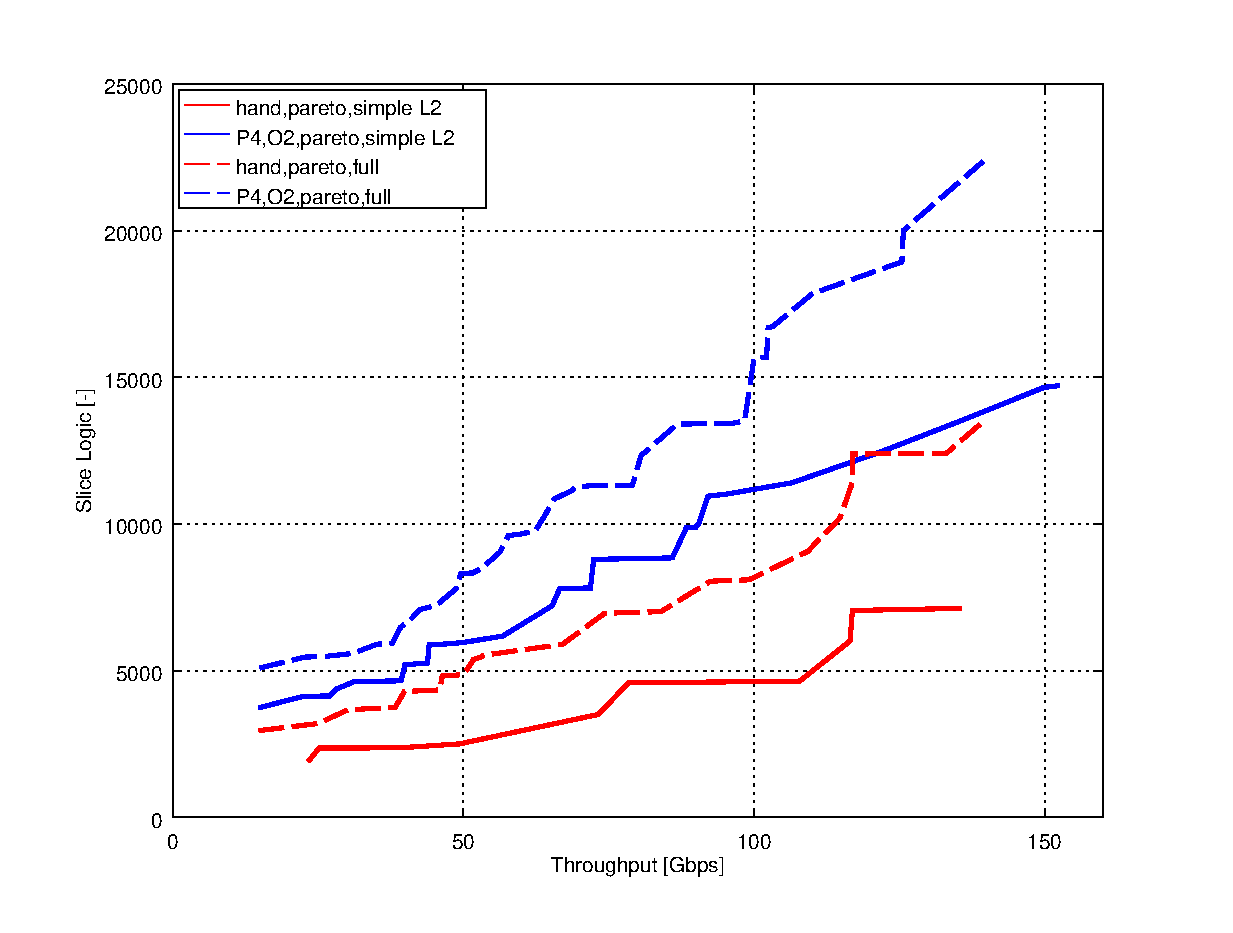
\includegraphics[width=0.89\textwidth]{pic/graph/hfe/1_thrslice_logic_pareto}
    \end{figure}
\end{frame}

\begin{frame}
    \frametitle{Parser --- Latency}
    \framesubtitle{Hand-written vs. Generated Parsers (the same protocol set)}
    
    \begin{figure}[t]
        \centering
        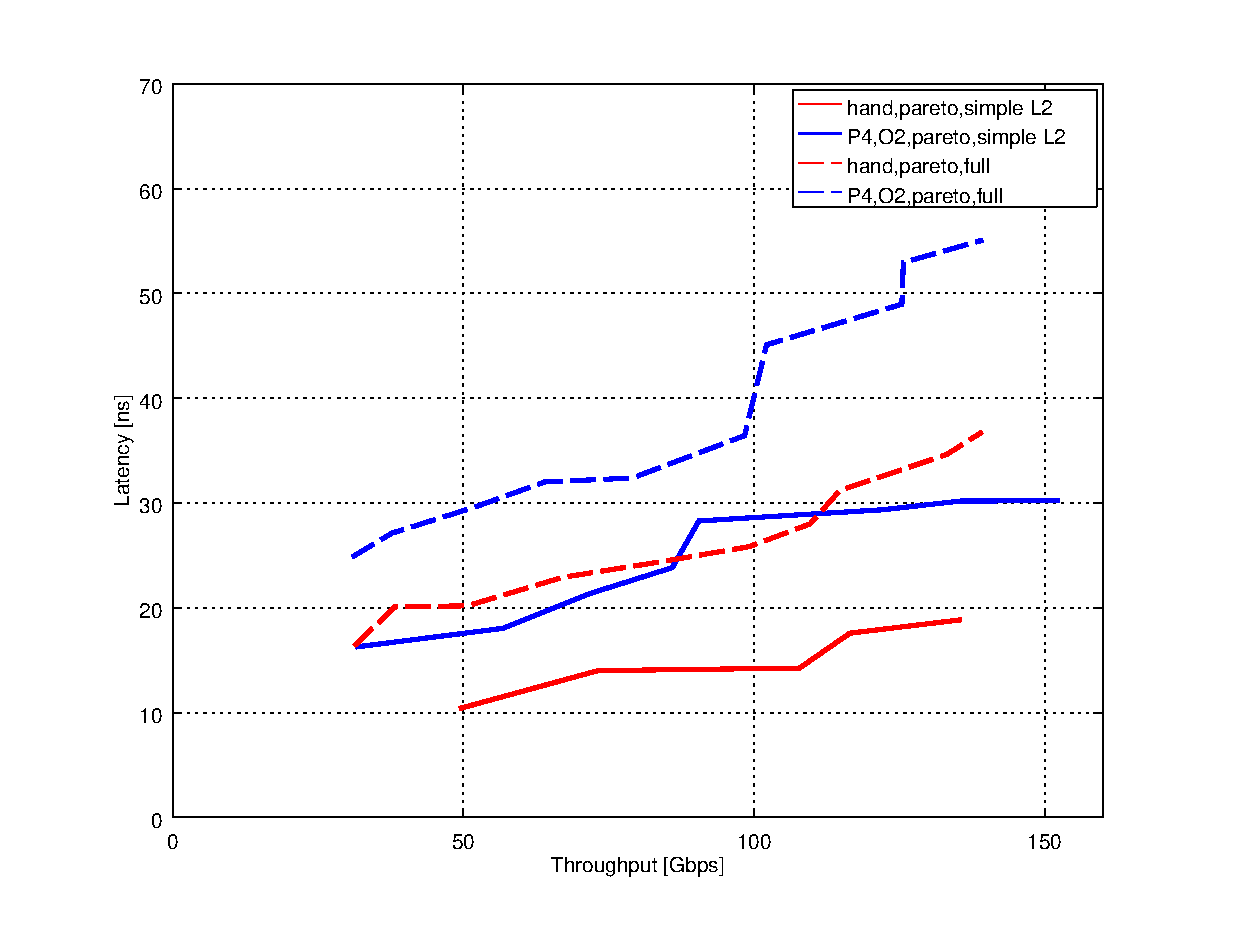
\includegraphics[width=0.89\textwidth]{pic/graph/hfe/2_thrlat_pareto}
    \end{figure}
\end{frame}

\subsection*{Deparser}
\begin{frame}
    \frametitle{Deparser}
    \framesubtitle{Published in [H2RC16], [P4ST16], [MICPRO16] journal}
    \begin{itemize}
        \fitem Deparsing $\rightarrow$ the reverse operation to parsing
        %\fitem In my best knowledge, I provided the first architecture and experimental results 
        \fitem I provided the following:
        \begin{itemize}
            \fitem Architecture of fundamental building blocks (configured and generated)
            \fitem The process of mapping from P4 to fundamental building blocks
        \end{itemize}
        
        \fitem The deparsing process is optimized to minimize consumed resources
        \begin{itemize}
            \fitem Protocol header is inserted \textbf{before} the payload
            \fitem Protocol with \textbf{fixed} length (e.g., Ethernet) --- shifting logic is simple
            \fitem Protocol with \textbf{variable} length (e.g., IPv4) --- shifting logic has to support several offsets for payload
        \end{itemize}
        
        \fitem The current architecture of deparser is inefficient when deparsing short frames 
    \end{itemize}
\end{frame}

\begin{frame}
    \frametitle{Deparser --- Consumed Resrouces}
    \framesubtitle{Generated Deparsers}
    
    \begin{figure}[t]
        \centering
        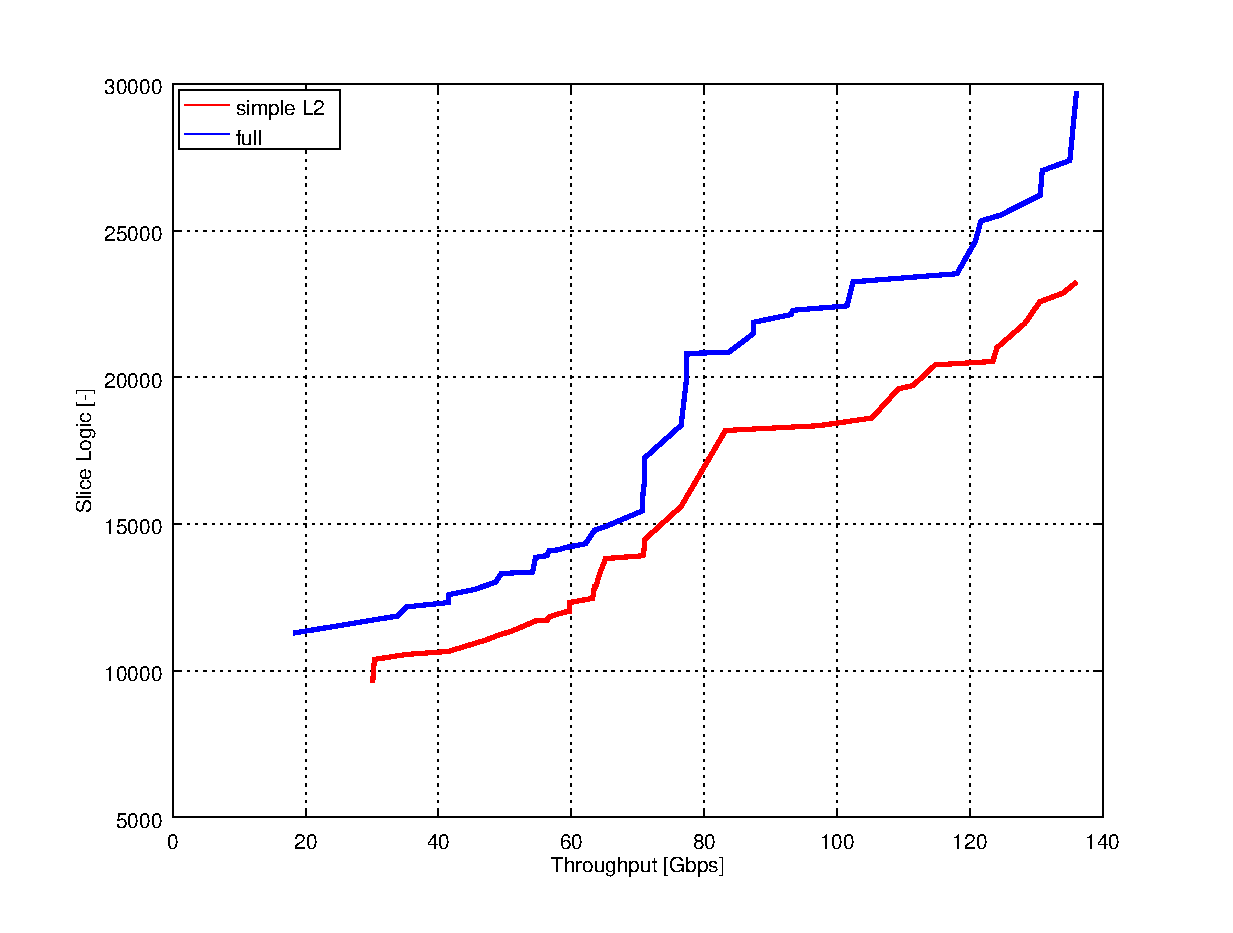
\includegraphics[width=0.89\textwidth]{pic/graph/deparser/1_thr_slice_logic_pareto}
    \end{figure}
\end{frame}

%\begin{frame}
%    \frametitle{Deparser --- Latency}
%    \framesubtitle{Generated Deparsers}
%    
%    \begin{figure}[t]
%        \centering
%        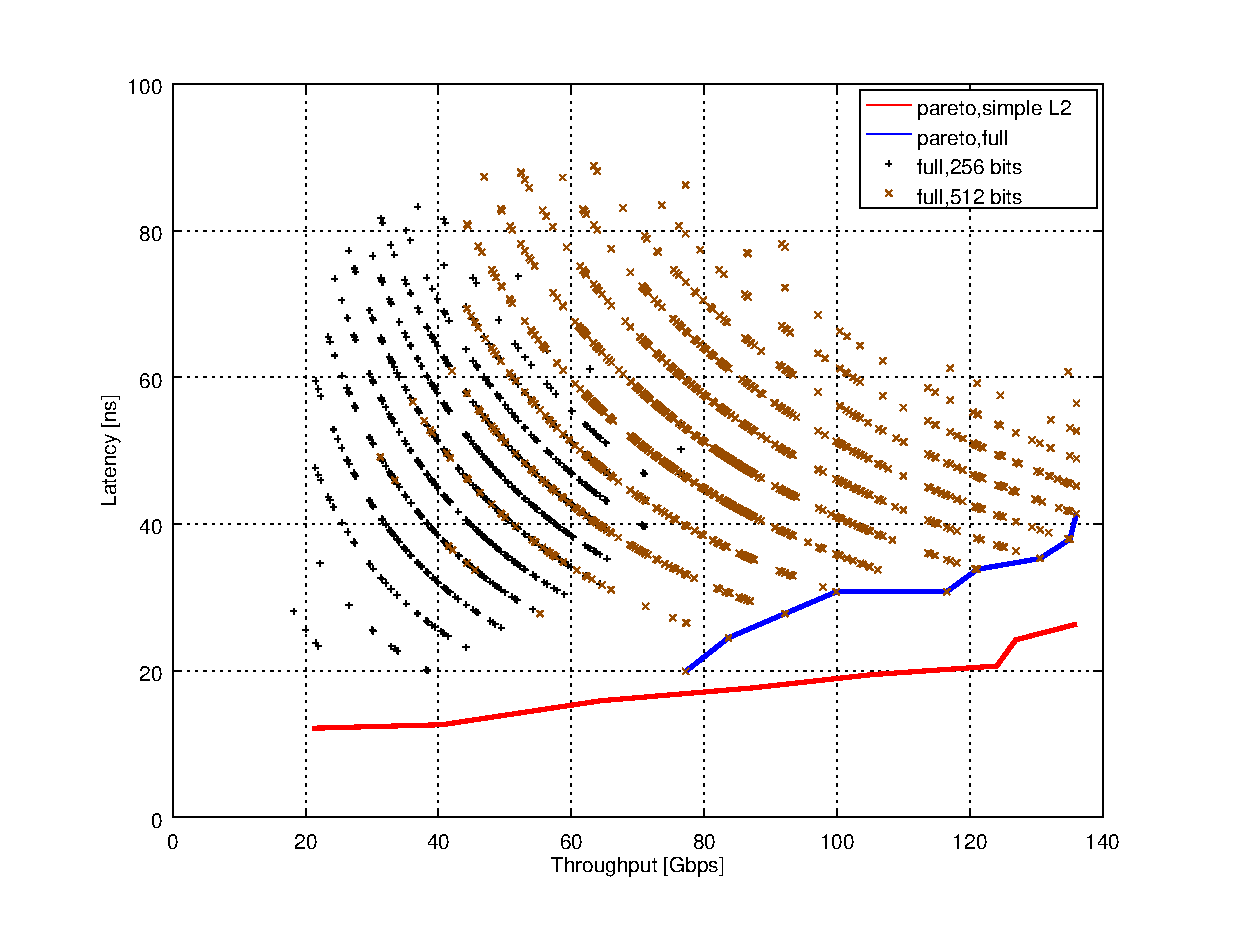
\includegraphics[width=0.89\textwidth]{pic/graph/deparser/3_thr_latency_deparser}
%    \end{figure}
%\end{frame}

\subsection*{Match+Action}
\begin{frame}
    \frametitle{Match+Action}
    \framesubtitle{Published in [MICPRO16], [H2RC16], [FPL13], [ANCS14], [MEMICS14], [FPGA14]}
    
    %\todo{Sem dat info o match+action, prvni implementace, mapovane komplet z vhdl, propustnost 100gbps, ukazano na trech use casech}
    \begin{itemize}
        \fitem Implements the \textbf{Match} (i.e., searching for the most suitable rule) and \textbf{Action} (i.e., data modification) functionality
        \begin{itemize}
            \fitem Search algorithms are out of scope of my work
        \end{itemize}
        %
        \fitem Modular architecture of Match+Action pipeline, designed to process 100\,Gbps and beyond
        \fitem I provided the following:
        \begin{itemize}
            \fitem Architecture of fundamental building blocks (configured, generated and mixed)
            \fitem The process of mapping from P4 to fundamental building blocks
        \end{itemize}
        %
        \fitem Optional usage of HLS for easy extensibility of action set
        \begin{itemize}
            \fitem Based on my research for DMON100 project\footnote{More information available from \url{http://dmon100.liberouter.org/}}
            \fitem I use C/C++ for description of complex processing at speed of 100\,Gbps
            \fitem Allows us extend the action set of P4 language in shorter time
        \end{itemize}
        %
        %\fitem Experiments --- to address consumed resources and throughput of generated P4 pipelines
    \end{itemize}
\end{frame}

\begin{frame}
    \frametitle{Generated P4 Pipelines --- Consumed Resources}
    \framesubtitle{Published in [MICPRO16] journal,[H2RC16]}
    
    \begin{figure}
        \centering
        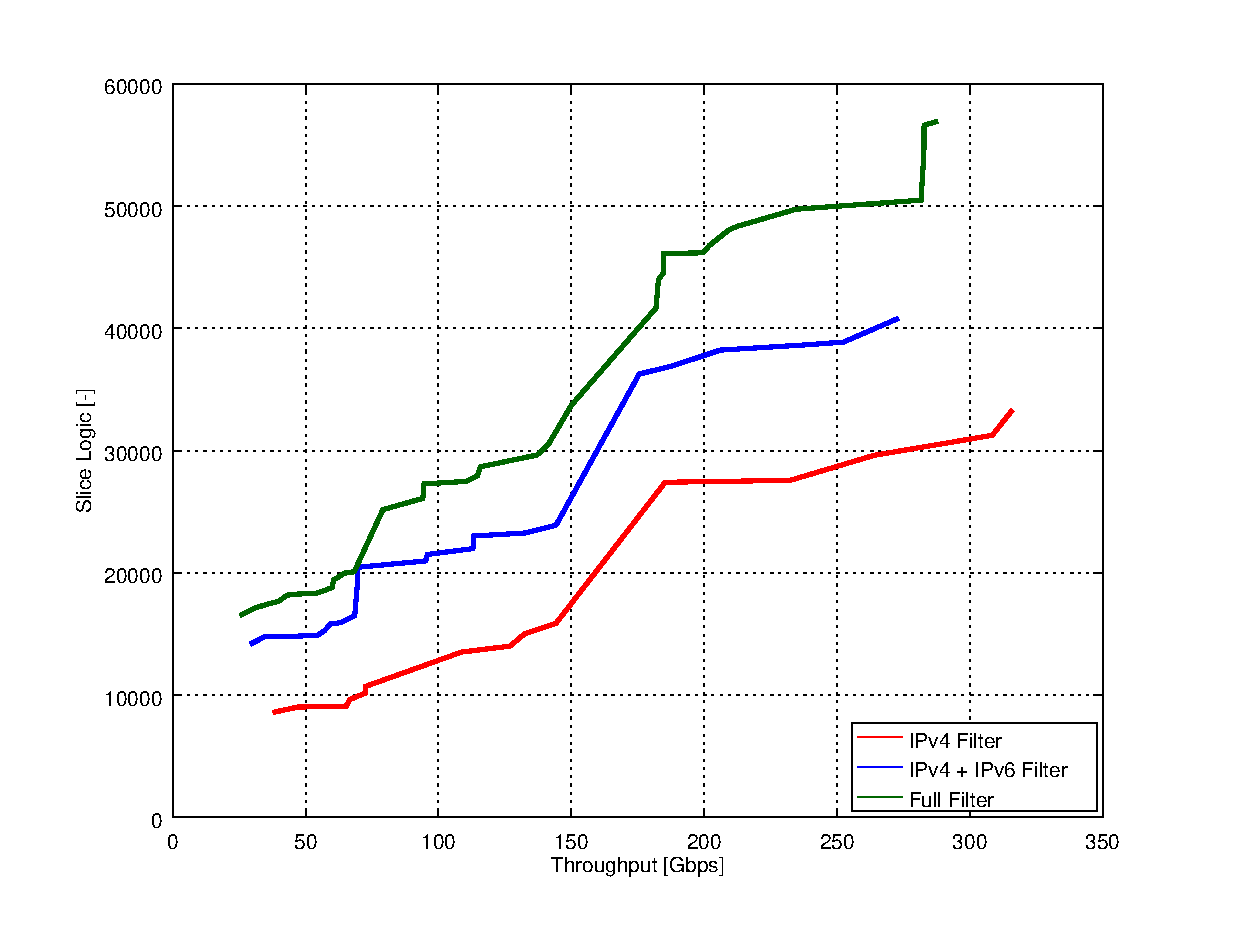
\includegraphics[width=0.89\textwidth]{pic/graph/table/thr_slice_logic_pareto}
    \end{figure}
\end{frame}

\begin{frame}[allowframebreaks]
    \frametitle{Generated P4 Pipelines --- Throughput}
    \framesubtitle{Published in [MICPRO16] journal}
    
    \begin{figure}
        \centering
        \includegraphics[width=0.89\textwidth]{pic/graph/table/ipv46_throughput}
    \end{figure}
    
    \begin{figure}
        \centering
        \includegraphics[width=0.89\textwidth]{pic/graph/table/detail_throughput_ineff}
    \end{figure}
\end{frame}

\subsection*{Comparison with Related Work}
\begin{frame}
    \frametitle{Comparison with Related Work}
    \framesubtitle{P4 $\rightarrow$ Bluespec}
    \begin{itemize}
        \fitem The nearest comparable solution: mapping P4 $\rightarrow$ Bluespec\footnote{More information available from \url{http://www.bluespec.com/}}
        \begin{itemize}
            \footnotesize
            \fitem[$\rightarrow$] Wang, Han, et al. \textit{P4FPGA: A Rapid Prototyping Framework for P4}. ACM SOSR 2017 Symposium on SDN research, Santa Clara, CA, USA, 2017.
        \end{itemize}
        %
        \fitem Their solution:
        \begin{itemize}
            \fitem Supports both versions of P4 language (P4\textsubscript{14} and P4\textsubscript{16})
            \fitem Supports API for easy configuration of network device
            \fitem Supports simple stateful processing
            \fitem No demonstration of advanced deparsing
        \end{itemize}
        \fitem My solution:
        \begin{itemize}
            \fitem Higher throughput (60\,Gbps vs. 100\,Gbps and beyond)
            \fitem No additional tool is needed (Bluespec $\rightarrow$ Verilog)
            \fitem Capable to reach higher frequencies on slower FPGA
            \fitem Throughput of parser is protocol independent
        \end{itemize}
            
    \end{itemize}
\end{frame}
